\section{卷积积分}

\subsection{信号的时域分解与卷积积分}

\begin{BoxDefinition}[信号的时域分解]*
    对于任意的信号,均可以用若干个冲激函数叠加表示。

    定义$p(t)$如下图
    \begin{figure}[H]
        \centering
        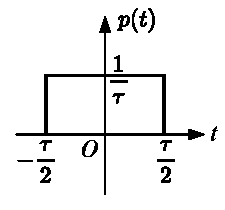
\includegraphics[width=30mm]{visio/2.1.pdf}
    \end{figure}
    
    则对于任意函数,有

    \begin{Equation}
        \hat{f} (t) = \sum\limits_{k=-\infty}^{\infty}f(k\Delta\tau) \cdot \Delta\tau \cdot p(t-k\Delta\tau)
    \end{Equation}

    因此

    \begin{Equation}
         f(t) = \lim\limits_{\Delta\tau\rightarrow 0}\hat{f} (t) = \int_{-\infty}^{\infty}f(\tau) \delta(t-\tau) d\tau
    \end{Equation}


\end{BoxDefinition}

\begin{BoxDefinition}[卷积积分]
    已知定义在区间$(-\infty,\infty)$上的两个函数$f_1(t)$和$f_2(t)$,则定义积分
    \begin{Equation}
        f(t) = \int_{\infty}^{\infty} f_1(\tau)f_2(t-\tau)d\tau
    \end{Equation}
    为$f_1(t)$和$f_2(t)$的卷积积分,简称卷积。记为
    \begin{Equation}
         f(t) = f_1(t)*f_2(t)
    \end{Equation}
    例如对于$y_{zs}(t)$
    \begin{Equation}
        y_{zs}(t) = \int_{\infty}^{\infty}f(\tau)h(t-\tau)d\tau = f(t)*h(t)
    \end{Equation}
    
\end{BoxDefinition}

\subsection{卷积的图解法}

\begin{BoxProperty}[卷积的图解法]*
    对于卷积积分
    \begin{Equation}
        f(t) = \int_{-\infty}^{\infty} f_1(\tau)f_2(t-\tau)d\tau
    \end{Equation}
    图解法求卷积过程可分解为四步:

    第一步换元
    \begin{Equation}
        t\rightarrow\tau \Rightarrow f_1(\tau),f_2(\tau)
    \end{Equation}
    第二步反转平移(画出$f_1(t)$和$f_2(t-\tau)$的图像\footnote{此处$\tau$带负号,因此$t>0$时图像右移,$t<0$时图像左移})
    \begin{Equation}
        f_2(\tau) \rightarrow f_2(-\tau) \rightarrow f_2(t-\tau)
    \end{Equation}
    第三步将信号重叠部分相乘(分类讨论区间),列出对应式子。

    第四步按分类讨论的区间将相乘后的图形进行积分。

    若求某一时刻的卷积积分值,反转平移步骤直接平移对应单位后相乘积分即可。
    
\end{BoxProperty}
